%%%%%%%%%%%%%%%%%%%%%%%%%%%%%%%%%%%%%%%%%%%%%%%%%%%%%%
\chapter{General introduction}
\label{general_introduction}
\graphicspath{{chapter_01/figures}{chapter_01/tables}}
%%%%%%%%%%%%%%%%%%%%%%%%%%%%%%%%%%%%%%%%%%%%%%%%%%%%%%



\chapterindent Flash \marginpara{The socio-economic impacts of flash floods} floods represent the deadliest and most devastating form of natural hazard, causing over 5,000 fatalities annually and accounting for approximately 85\% of global flood incidents \citep{Dordevic_2020}. The impact of flash floods extends across urban and rural landscapes, profoundly affecting lives, livelihoods, and critical infrastructure worldwide \citep{Liu_2024a}. The socio-economic \citep{Ebi_2021} and environmental \citep{Zhang_2024a} impacts of flash floods can be severe and transcend the traditional divide

\vspace*{\fill}
\begin{tcolorbox}[
  colframe=colour_body_text,
  colback=white,
  sharp corners,
  boxrule=2mm,
  left=0mm,
  right=0mm,
  toprule=0mm,
  bottomrule=0mm,
  rightrule=2mm
]
{\color{colour_body_text} 
\textbf{DEFINITIONS CONSIDERED IN THIS THESIS}

\vspace{1em}
\textbf{\uline{Flash Flood}}\newline
Two types of flash floods are considered: \textit{fluvial flash floods}, defined as a rapid water level rise in a stream or creek above a predetermined flood level \citep{NWS_2024}; and \textit{pluvial flash floods}, defined as flooding resulting from rainfall when water ponds or flows over the ground before it enters a natural or man-made drainage system or watercourse, or when it cannot enter because the system is already full to capacity \citep{Speight_2021}. For both types of flash floods, flooding is considered to occur within a few hours of the causative event. In this thesis, the only considered causative event is rainfall.

\vspace{1em}
{\textbf{\uline{Area at Risk of Flash Floods}}\newline
It refers to a polygon - or area - that might experience flash flooding due to the expected rainfall.
}
\end{tcolorbox}
\vspace{0pt}

\noindent between developed and developing countries. In October 2024, flash floods in Valencia, Spain, claimed more than 200 lives and caused extensive damage in 87 municipalities \citep{Grau-Bove_2024}, while between March and September 2024, sustained periods of intense rainfall and subsequent flash flooding in Pakistan and Afghanistan resulted in 1084 deaths, 2600 injuries, and extensive damage to houses \citep{Wikipedia_2025}. In low- and middle-income countries in Africa, Latin America, and Asia, flash floods can also exacerbate existing socio-economic and environmental vulnerabilities to the extent of displacing entire populations \citep{Stephens_2024} or undermining food security and food safety \citep{Agabiirwe_2022, Duchenne-Moutien_2021}. Impacts from flash floods are more severe primarily due to rapid, unregulated urbanisation in flood-prone areas, limited infrastructure for flood management, insufficient early warning systems, and economic constraints on implementing preventive measures \citep{Douglas_2017, Pinos_2022, Wang_2021b}. Regions affected by flash floods can also be vulnerable to waterborne diseases, with outbreaks of cholera, typhoid, and other infectious diseases occurring when floodwaters contaminate drinking water sources or overwhelm sanitation systems \citep{Lee_2020}. Populations affected by extremely severe flash floods may also experience serious psychological impacts, including anxiety, depression, and post-traumatic stress disorder \citep{Iqbal_2023}. 

As \marginpara{On the urgent need for accurate, timely, and scalable flash flood forecasts} climate change increases the frequency and intensity of extreme rainfall \citep{WMO_2025, IPCC_2023}, also in historically low-risk regions \citep{Fowler_2021c}, a comprehensive re-evaluation of risk management, adaptation, and mitigation frameworks is needed to protect vulnerable communities. Recognising their severe and growing impacts, WMO targets flash floods as one of its top priority natural hazards \citep{WMO_2025}. The UN's 'Early Warnings for All' initiative, launched in 2022, which aims to protect every person on Earth with early warning systems by 2027, places flash floods at the forefront of its agenda \citep{UN_2022}. Forecasts with global coverage that are accurate and timely (e.g. several days in advance) are crucial to the success of such an initiative as they could enable targeted protective decisions worldwide \citep{Merz_2020}, including in regions where longer lead times are crucial for mobilising resources and executing emergency plans \citep{Bazo_2019}. 

Despite \marginpara{Current challenges in flash flood forecasting: scaling predictions for large domains and extending lead times} general advances in flash flood prediction (for example, the development of high-resolution physical and data-driven NWP and hydrological models), significant technical and methodological obstacles persist for the development of medium-range flash flood forecasts (i.e. up to 5 days ahead), over a continuous global domain \citep{Zanchetta_2020}. Such obstacles include inherent uncertainty in extreme, localised rainfall forecasts beyond a few hours, computational demands of running high-resolution models over large domains, and the limited availability of real-time hydro-meteorological observations. These limitations hinder the ability to predict flash floods with sufficient lead time and across a large-scale, continuous domain (e.g., global), leaving many regions unprotected \citep{AlRawas_2024}. The WMO's Flash Flood Guidance System attempts to address the patchy spatial coverage of flash flood forecasting systems \citep{Georgakakos_2022}. This initiative, however, focuses on implementing distinct regional systems around the world, not resolving the issue of spatial patchy coverage. Furthermore, the system's reliance on high-density observational networks, km-scale NWP model outputs, and high computational costs compromises scalability of the project in regions with limited resources. Therefore, developing robust medium-range flash flood forecasting capabilities on a global scale remains one of the pressing challenges in modern hydrology.

The \marginpara{Opportunities for global medium-range flash flood forecasts: proven effectiveness of index-based systems over large-scale domains, enhanced quality of medium-range global NWP rainfall predictions, and emergence of data-driven approaches for hydrological applications} unprecedented convergence of three key scientific advancements over the last decade has created a unique opportunity to develop medium-range flash flood forecasts with global coverage. First, index-based flash flood forecasting systems, focusing on key variables such as rainfall and soil moisture, have proven more effective and computationally efficient at national and continental scales than complex physically-based models \citep{Alfieri_2015a}. However, their reliance on high-resolution, short-range rainfall forecasts from radars or km-scale NWP models still limits their spatial coverage to data-rich regions like Europe and the US, and restricts forecasts lead times to nowcasting time scales (i.e. a few hours), thereby reducing available preparedness and response time \citep{Luong_2021, Maybee_2024}. Second, over the past decade, global (ensemble) NWP models have significantly improved their ability to forecast extreme rainfall up to the medium-range lead times \citep{Lavers_2021, Haiden_2023}. Despite their coarse spatial resolution (typically >10 km), there is growing interest in testing global NWP forecasts for flash flood applications and extending prediction lead times \citep{Bucherie_2022b}. Moreover, statistical post-processing techniques make these predictions more palatable for flash flood forecasting \citep{Vannitsem_2021}. Third, the recent success of data-driven approaches in predicting riverine floods \citep{Nearing_2024} has increased the interest in extending their application to flash flood forecasting. Notwithstanding the innovative paradigm of \textit{training a model where data is available and applying it globally} \citep{Kratzert_2024}, the paucity of observational data suitable for flash flood modelling continues to hinder the development of data-driven approaches for large-scale flash flood forecasting \citep{Alzubaidi_2023}. When run using global medium-range NWP model outputs, simpler machine learning models (e.g., decision-tree-based algorithms or feed-forward neural networks), optimised for sparse and imbalanced datasets, and informed by physical insights from index-based models, may enable the development of a proof-of-concept for medium-range data-driven hydro-meteorological predictions of areas at risk of flash floods with true global coverage.


%%%%%%%%%%%%%%%%%%%%%%%%%%%%%%%%%%%%%%%%%%%%%%%%%%%%%%%%%%%%%%%%%%%%%%%%%%%
\section{Research questions and objectives, and contributions to knowledge}
\label{general_introduction_research_questions_objectives_contribution2knowledge}

While \marginpara{Development of flash-flood-focused verification framework and establishment of rainfall-based performance benchmark for comparative assessment against more sophisticated predictions of areas at risk of flash floods} new global NWP rainfall forecasts are regularly developed, their effectiveness in identifying areas at risk of flash floods remains largely untested. Most verification efforts compare predicted rainfall against rainfall observations, implicitly assuming that improved rainfall forecasts will translate into better flash flood prediction capabilities \citep{Gascón_2024}. However, this assumption requires direct validation through a flash-flood-focused assessment. 

\begin{tcolorbox}[
  colframe=colour_chapter5,  
  colback=white,           
  sharp corners,        
  boxrule=2mm,          
  left=0mm,             
  right=0mm,            
  toprule=0mm,          
  bottomrule=0mm,       
  rightrule=2mm        
]
{\color{colour_chapter5} {\setlength{\parindent}{1.0em} Research Question n.1 (RQ1): Can post-processed global NWP rainfall forecasts successfully identify areas at risk of flash floods up to medium-range lead times?}}
\end{tcolorbox}

\noindent To address RQ1, the \uline{first research objective} of this thesis involves departing from the traditional rainfall-to-rainfall verification approach and adopting, instead, a \textit{flash-flood-focused verification framework} that directly compares rainfall forecasts with flash flood impact reports - to encompass fluvial and pluvial flash flood events. This framework must overcome two main methodological challenges: addressing spatio-temporal uncertainties in flash flood reports, and establishing meaningful performance measures that account for the inherent rarity of flash flood events and the differences between continuous rainfall predictions and binary flash flood occurrence (as measured by impact reports). \uline{Addressing RQ1 delivers two fundamental contributions to knowledge}. First, it establishes a performance baseline by evaluating state-of-the-art global NWP rainfall forecasts against flash flood impact reports, providing a quantitative benchmark against which more sophisticated predictions (e.g., incorporating hydro-meteorological parameters) can be assessed. Second, the framework itself constitutes a contribution - a standardised assessment tool applicable to any flash flood prediction, whether rainfall-based or hydro-meteorological, physical or data-driven. This versatile framework will underpin all subsequent verification analyses in this thesis, enabling systematic comparison across increasingly complex prediction methodologies.

Data-driven \marginpara{Development of data-driven hydro-meteorological predictions of areas at risk of flash floods up to medium-range lead times} models \citep{Nearing_2024} and large-sample hydrology \citep{Kratzert_2024} have recently transformed riverine flood prediction, yet data-driven flash flood prediction remains confined at catchment/regional or \citep{Song_2020, Saleh_2024, Ding_2025, Zhao_2025} or national scale \citep{Zhao_2022}, and forecast lead times rarely exceed 24 hours. The development of medium-range, global data-driven flash flood prediction systems faces a fundamental obstacle: severe class imbalance between flash flood and non-flood events in observational datasets for this hazard. This severe imbalance - stemming from the inherent rarity of flash flood events, the predominant number of ungauged flashy catchments, and the systematic underreporting of this hazard in global impact databases - restricts flash flood observations to <1\% of records in global datasets \citep{Panwar_2020, Kratzert_2023, Färber_2024, Jonkman_2024}.

\begin{tcolorbox}[
  colframe=colour_chapter6,  
  colback=white,           
  sharp corners,        
  boxrule=2mm,          
  left=0mm,             
  right=0mm,            
  toprule=0mm,          
  bottomrule=0mm,       
  rightrule=2mm        
]
{\color{colour_chapter6} {\setlength{\parindent}{1.0em} Research Question n.2 (RQ2): Are medium-range data-driven hydro-meteorological predictions of areas at risk of flash floods feasible with global reanalysis, forecasts, and impact flash flood reports?
}}
\end{tcolorbox}

\noindent To address RQ2, the \uline{second research objective} of this thesis involves developing data-driven models that integrate hydro-meteorological variables from global reanalysis and global medium-range NWP forecasts, and flash flood impact reports to predict areas at risk of flash floods, from short- (i.e., day 1) to medium-range lead times (i.e., day 5). This development must overcome three methodological challenges: selecting architectures that handle severe class imbalance effectively - where parsimonious approaches, such as regularised ensemble methods and shallow neural networks, may outperform deep learning \citep{Kumar_2021, Xu_2022, Luo_2025a}; feature engineering that balance informativeness, interpretability, and computational efficiency when identifying key hydro-meteorological variables; building ensemble models to quantifying uncertainty and provide reliable risk estimates \citep{Saleh_2024}. \uline{Addressing RQ2 delivers two fundamental contributions to knowledge}. First, it establishes the feasibility and predictability limits of medium-range data-driven predictions of areas at risk of flash floods. Second, it demonstrates whether more sophisticated predictions, integrating hydro-meteorological parameters and complex probabilistic data-driven approaches, enhance the predictive capability of identifying areas at risk of flash floods up to medium-range lead times compared to the rainfall-only baseline established in RQ1. 

The \marginpara{Systematic empirical evaluation of training data strategies for global predictions of areas at risk of flash floods under varying spatial coverage and data density scenarios.} verification analysis and data-driven model development presented in the previous paragraphs focused on a regional domain with high-quality, high-density flash flood impact reports. Even though these regionally-trained data-driven models may demonstrate strong performance within the considered domain, this thesis aims to develop a proof-of-concept for predicting areas at risk of flash floods \textit{over a continuous global domain}. The lack of high-density global flash flood impact databases \citep{Panwar_2020} creates a fundamental tension between two contrasting approaches for developing predictions of areas at risk of flash floods with a continuous global coverage: training models on sparse but global datasets versus leveraging high-quality regional observations and applying the trained model globally, as suggested by \citet{Kratzert_2024}. 

\begin{tcolorbox}[
  colframe=colour_chapter7,  
  colback=white,           
  sharp corners,        
  boxrule=2mm,          
  left=0mm,             
  right=0mm,            
  toprule=0mm,          
  bottomrule=0mm,       
  rightrule=2mm        
]
{\color{colour_chapter7} {\setlength{\parindent}{1.0em} Research Question n.3 (RQ3): How does coverage-density trade-off influence training data strategies to develop predictions of areas at risk of flash floods over a continuous global domain?}}
\end{tcolorbox}

\noindent To address RQ3, the \uline{third research objective} of this thesis involves the assessment - through a systematic empirical sensitivity analysis - of how varying spatial coverage and data density scenarios may influence training data strategies when creating global predictions with regionally-trained data-driven models (as those developed to address RQ2). This investigation must overcome two primary challenges: quantify how performance degrades across different sensitivity analysis configurations to identify the optimal trade-off between geographical coverage and data quality, and establish subjective validation protocols for regions lacking comprehensive flash flood databases. \uline{Addressing RQ3 delivers two fundamental contributions to knowledge}. First, it provides empirical evidence quantifying how different training data strategies — from sparse global coverage to dense regional coverage — may influence the accuracy of global predictions. Second, it assesses whether regionally-trained models can maintain meaningful predictive skill when applied to data-scarce regions outside the training domain. This evidence supports a pragmatic pathway toward global flash flood early warning systems, particularly valuable for regions where traditional forecasting approaches face data or resource limitations. Moreover, the outcomes of this research would align with the UN's "Early Warnings for All" initiative by potentially extending life-saving warnings to historically underserved communities.

 
%%%%%%%%%%%%%%%%%%%%%%%%%%%%%%%%%%%%%%%%%%%
\section{Thesis structure}
This thesis is divided into the following nine chapters:

\begin{figure}[htbp]
\centering
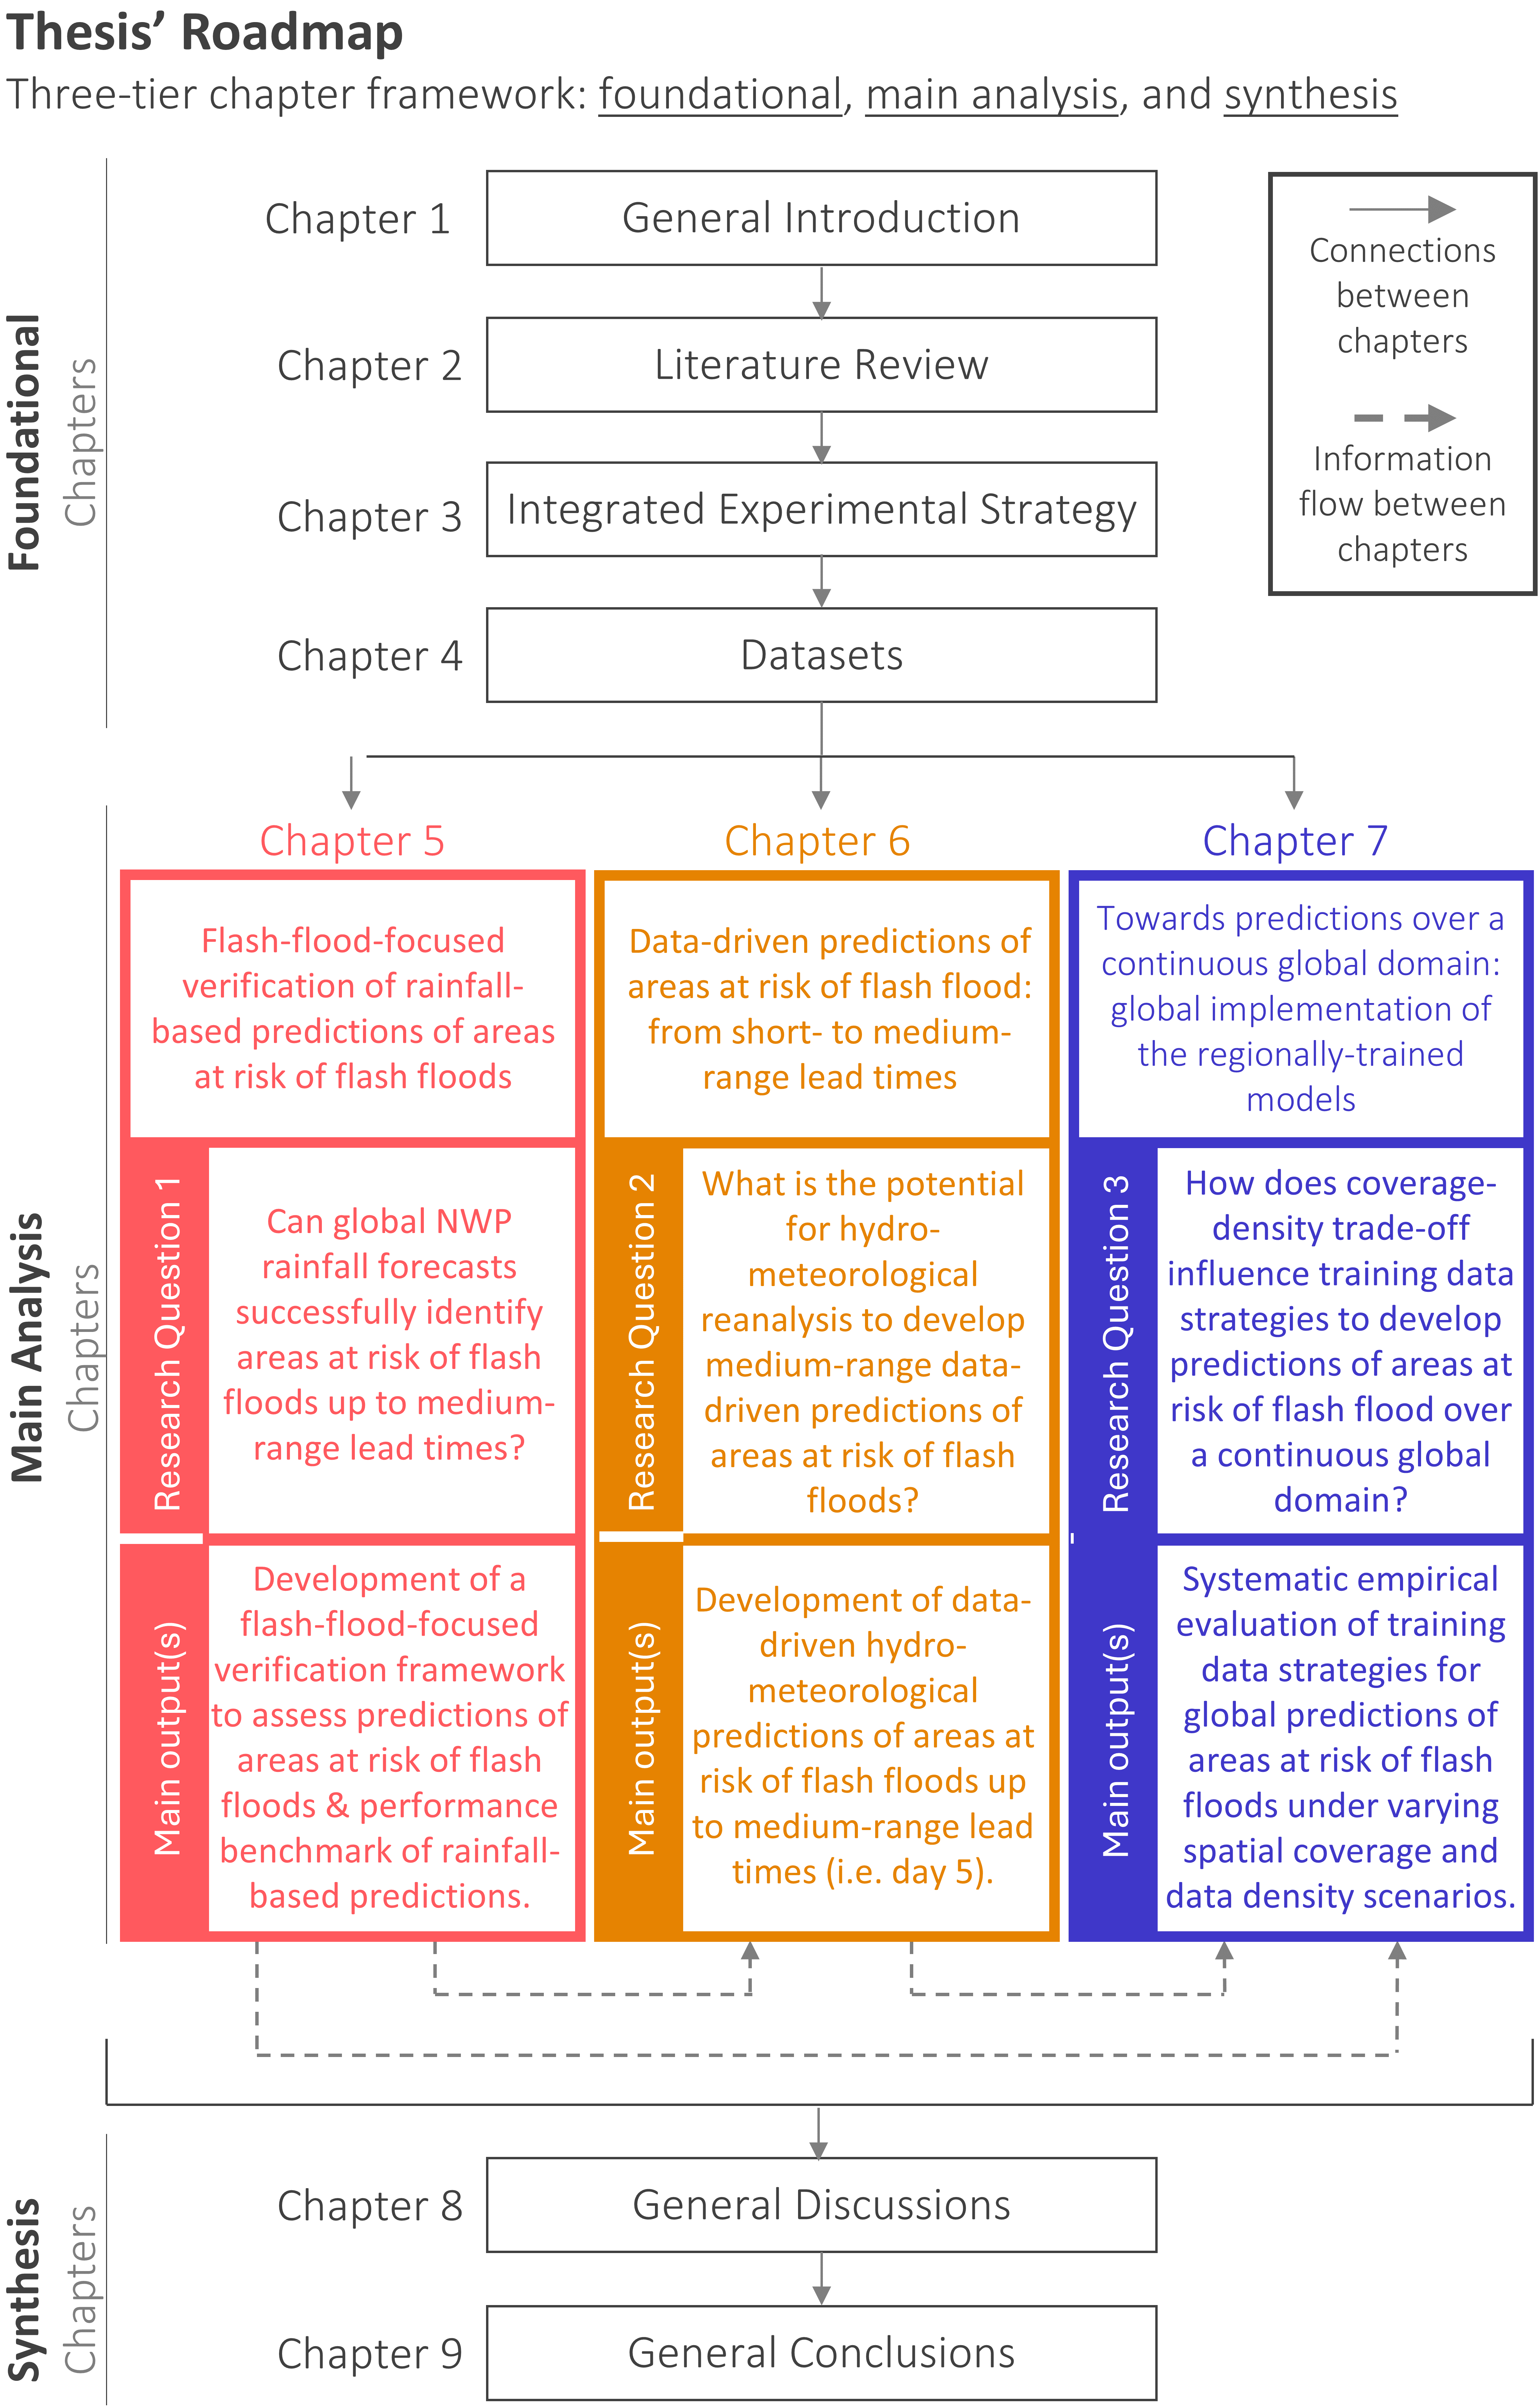
\includegraphics[width=\textwidth]{thesis_roadmap.png}
\caption{\textbf{Thesis' roadmap.} Three-tier chapter framework comprising \textbf{Foundational} Chapters (Chapter 1-4: General Introduction, Literature Review, Integrated Experimental Strategy, and Datasets), \textbf{Main Analysis} Chapters (\textcolor{colour_chapter5}{Chapter 5: Development of a flash-flood-focused verification framework}; \textcolor{colour_chapter6}{Chapter 6: Development of medium-range data-driven hydro-meteorological predictions of areas at risk of flash floods}; \textcolor{colour_chapter7}{Chapter 7, blue: Global implementation of regionally-trained data-driven models}), and \textbf{Synthesis} Chapters (Chapter 8-9: General Discussions and General Conclusions). Research questions and main output(s) are indicated for each main analysis chapter.}
\label{fig:thesis_structure}
\end{figure}

\textbf{Chapter 1}\marginpara{Foundational Chapter - General Introduction} established the foundation for this research by addressing the critical need for improved flash flood early warning systems worldwide. The chapter presented the three interconnected research questions and objectives addressed in this thesis, and introduced the contributions to knowledge made by this thesis - which will be discussed in more detail in Chapter \ref{general_discussions}.

\textbf{Chapter 2}\marginpara{Foundational Chapter - Literature Review} will present a synthesis of the scientific literature in flash flood prediction, establishing the theoretical foundations that delineate the methodological gaps addressed by the three research questions presented in Section \ref{general_introduction_research_questions_objectives_contribution2knowledge}.

\textbf{Chapter 3}\marginpara{Foundational Chapter - Integrated Experimental Strategy} delineates the integrated experimental strategy through which the three research questions are systematically addressed, demonstrating their dependencies and relationships.

\textbf{Chapter 4}\marginpara{Foundational Chapter - Datasets} presents the datasets considered to address the three presented research questions. It presents the flash flood impact database used throughout this thesis - NOAA's Storm Event Database - discussing its geographical and temporal coverage, as well as its inherent strengths and limitations. The chapter also describes the hydrological and static parameters from ERA5 - reanalysis and medium-range forecasts - used in this thesis. It finally presents the characteristics of the ERA5-ecPoint rainfall - reanalysis and medium-range forecasts - used in this thesis to enhance the representation of localised extreme flash-flood-triggering rainfall events.

\textbf{Chapter 5}\marginpara{\textcolor{colour_chapter5}{Main Analysis Chapter - Flash-flood-focused verification of rainfall-based predictions of areas at risk of flash floods}} addresses RQ1 by developing a flash-flood-focused verification framework - a standardised assessment tool applicable to diverse predictions of areas at risk of flash floods - and establishes a quantitative performance baseline for rainfall-based predictions against which more sophisticated predictions may be compared.

\textbf{Chapter 6}\marginpara{\textcolor{colour_chapter6}{Main Analysis Chapter - Data-driven hydro-meteorological predictions of areas at risk of flash flood: from short- to medium-range lead times}} addresses RQ2 by developing and evaluating multiple data-driven architectures trained on hydro-meteorological reanalysis data and run with medium-range global NWP hydro-meteorological forecasts to analyse forecast predictability. The chapter also demonstrates whether integrating additional variables enhances forecast performance compared to the rainfall-based benchmark.

\textbf{Chapter 7}\marginpara{\textcolor{colour_chapter7}{Main Analysis Chapter - Towards predictions over a continuous global domain: global implementation of the regionally-trained models}} addresses RQ3 by providing empirical evidence for optimal training data strategies to develop predictions of areas at risk of flash floods over a continuous global domain, and assessing coverage-density trade-offs through systematic sensitivity analysis.

\textbf{Chapter 8}\marginpara{Synthesis Chapter - General Discussions} synthesises and discusses the research findings in the main analysis chapters, critically evaluating how effectively each research question was addressed. The chapter examines the broader implications of the thesis's outcomes for flash flood risk reduction and emergency management, exploring how these advancements can enhance global early warning capabilities against the impacts of flash floods. 

\textbf{Chapter 9}\marginpara{Synthesis Chapter - General Conclusions} concludes the thesis by articulating its novel contributions to flash flood prediction knowledge and practice. It provides final assessments for each research question, acknowledging methodological limitations whilst clearly stating the scientific advancements achieved. The chapter concludes by exploring future research directions that could strengthen the use of forecasts from global NWP models and data-driven approaches for predicting flash floods over a continuous global domain and further extending forecast lead times. 